\section{Szkody, et al. (2002): Cataclysmic Variables from the Sloan Digital Sky Survey} \label{muestra:szkody2002}

Con el lanzamiento del SDSS, Szkody y su equipo reconocieron una nueva área de
oportunidad para expandir la población de variables cataclísmicas (VCs)
conocidas en la Galaxia. De interés particular son aquellos sistemas que más se
aproximan al periodo mínimo según los modelos evolutivos de las VCs; estos
objetos llegan a magnitudes fuera del alcance de la mayoría de los telescopios
usados hasta este entonces, por lo cual no han sido el objetivo de estudio en la
literatura. Partiendo de SDSS Szkody y colaboradores iniciaron una búsqueda de
VCs tenues, con la expectativa de capturar una muestra representativa de
variables cataclísmicas en nuestra galaxia, en particular obteniendo muestras de
poblaciones históricamente imperceptibles a nuestros instrumentos.

Para restringir los sistemas que buscar, Szkody y colaboradores aplicaron un
criterio de color basado en el trabajo de \citeyearparen{krisciunas1998SdssCriteria}, en
el cual lograron determinar concentraciones de diferentes tipos de objetos
utilizando diagramas de color-color. A pesar de haber hecho estas observaciones
antes del año de lanzamiento de SDSS, Krisciunas y colaboradores lograron
obtener observaciones utilizando equipo cuyas características se asemejan a las
de los instrumentos utilizados para SDSS. Partiendo de estos resultados, Szkody
y colaboradores determinaron criterios en las regiones azules y rojas del
espectro, cuyos valores se encuentran en las  
\refequations{muestra:szkody2002:criterioeqs}.

\begin{equation}
	\begin{split}
		& u^* - g^* < 0.45 \\
		& g^* - r^* < 0.7 \\
		& r^* - i^* > 0.30 \\
		& i^* - z^* > 0.4
	\end{split}
	\label{muestra:szkody2002:criterioeqs}
\end{equation}

Una vez recabada la muestra de candidatas a observar, Szkody y colaboradores
confirmaron su estatus como variables cataclísmicas basado en los espectros
obtenidos del SDSS desde el \textit{Apache Point Observatory}. Estos datos los
complementaron con observaciones de espectrografía con el telescopio de 3.5m en
el \textit{Apache Point Observatory} y observaciones fotométricas utilizando el
telescopio de 0.76m en el \textit{Manastash Ridge Observatory} de la Universidad
de Washington. En total identificaron 22 sistemas como variables cataclísmicas,
incluyendo 3 objetos previamente estudiados e identificados como tal. Presentan
la concentración de los objetos en el diagrama color-color, vistos en la
\reffigure{szkody2002ColorColorVCs}. 

\begin{figure}[!ht]
	\centering
	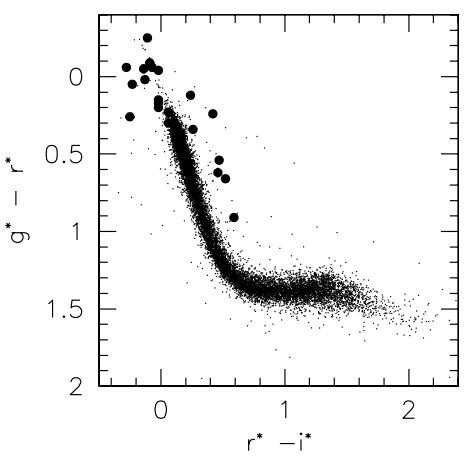
\includegraphics[scale=0.4]{Muestra/Secciones/Figures/gr-ri_Szkody2002.png}
	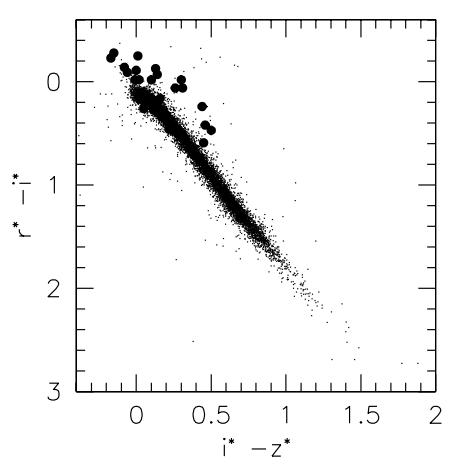
\includegraphics[scale=0.4]{Muestra/Secciones/Figures/ri-iz_Szkody2002.png}
	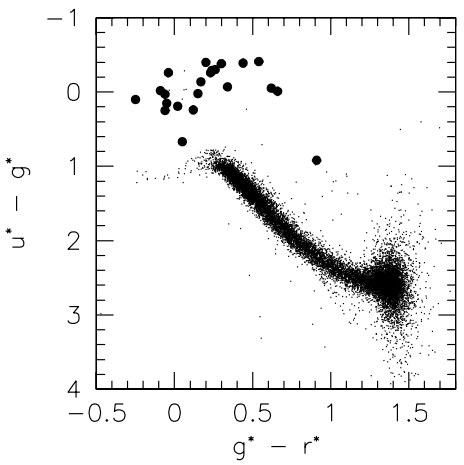
\includegraphics[scale=0.4]{Muestra/Secciones/Figures/ug-gr_Szkody2002.png}

	\caption{Variables cataclísmicas identificadas y observadas por Szkody y
		colaboradores (círculos negros fuertes). Se puede apreciar la separación
		de las variables cataclísmicas del locus estelar, vista en los puntos
		negros. \citeyearparen{szkody2002CvSearchSdss}}
	\label{szkody2002ColorColorVCs}
\end{figure}